\begin{figure}[H]
    \centering
    \tikzset{every picture/.style={line width=0.75pt}} %set default line width to 0.75pt        
    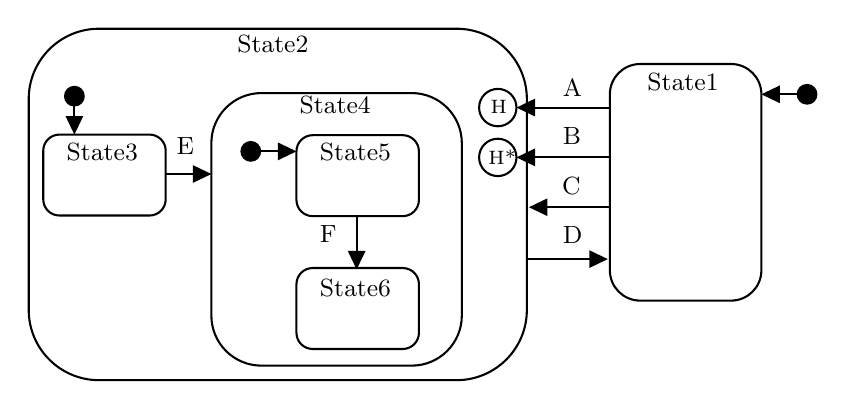
\begin{tikzpicture}[x=0.75pt,y=0.75pt,yscale=-1,xscale=1]
        \draw   (316,91.6) .. controls (316,83.54) and (322.54,77) .. (330.6,77) -- (374.4,77) .. controls (382.46,77) and (389,83.54) .. (389,91.6) -- (389,176.4) .. controls (389,184.46) and (382.46,191) .. (374.4,191) -- (330.6,191) .. controls (322.54,191) and (316,184.46) .. (316,176.4) -- cycle ;
        \draw   (36,93.87) .. controls (36,75.16) and (51.16,60) .. (69.87,60) -- (242.13,60) .. controls (260.84,60) and (276,75.16) .. (276,93.87) -- (276,195.47) .. controls (276,214.17) and (260.84,229.33) .. (242.13,229.33) -- (69.87,229.33) .. controls (51.16,229.33) and (36,214.17) .. (36,195.47) -- cycle ;
        \draw   (253,98) .. controls (253,93.03) and (257.03,89) .. (262,89) .. controls (266.97,89) and (271,93.03) .. (271,98) .. controls (271,102.97) and (266.97,107) .. (262,107) .. controls (257.03,107) and (253,102.97) .. (253,98) -- cycle ;
        \draw    (316,98) -- (274,98) ;
        \draw [shift={(271,98)}, rotate = 360] [fill=black][line width=0.08]  [draw opacity=0] (8.93,-4.29) -- (0,0) -- (8.93,4.29) -- cycle    ;
        \draw   (253,122) .. controls (253,117.03) and (257.03,113) .. (262,113) .. controls (266.97,113) and (271,117.03) .. (271,122) .. controls (271,126.97) and (266.97,131) .. (262,131) .. controls (257.03,131) and (253,126.97) .. (253,122) -- cycle ;
        \draw    (316,122) -- (274,122) ;
        \draw [shift={(271,122)}, rotate = 360] [fill=black][line width=0.08]  [draw opacity=0] (8.93,-4.29) -- (0,0) -- (8.93,4.29) -- cycle    ;
        \draw    (316,146) -- (280,146) ;
        \draw [shift={(277,146)}, rotate = 360] [fill=black][line width=0.08]  [draw opacity=0] (8.93,-4.29) -- (0,0) -- (8.93,4.29) -- cycle    ;
        \draw   (43,118.8) .. controls (43,114.49) and (46.49,111) .. (50.8,111) -- (94.2,111) .. controls (98.51,111) and (102,114.49) .. (102,118.8) -- (102,142.2) .. controls (102,146.51) and (98.51,150) .. (94.2,150) -- (50.8,150) .. controls (46.49,150) and (43,146.51) .. (43,142.2) -- cycle ;
        \draw   (124,115.13) .. controls (124,101.8) and (134.8,91) .. (148.13,91) -- (220.53,91) .. controls (233.86,91) and (244.67,101.8) .. (244.67,115.13) -- (244.67,198.2) .. controls (244.67,211.53) and (233.86,222.33) .. (220.53,222.33) -- (148.13,222.33) .. controls (134.8,222.33) and (124,211.53) .. (124,198.2) -- cycle ;
        \draw    (102,130) -- (121,130) ;
        \draw [shift={(124,130)}, rotate = 180] [fill=black][line width=0.08]  [draw opacity=0] (8.93,-4.29) -- (0,0) -- (8.93,4.29) -- cycle    ;
        \draw   (165,119.1) .. controls (165,114.79) and (168.49,111.3) .. (172.8,111.3) -- (216.2,111.3) .. controls (220.51,111.3) and (224,114.79) .. (224,119.1) -- (224,142.5) .. controls (224,146.81) and (220.51,150.3) .. (216.2,150.3) -- (172.8,150.3) .. controls (168.49,150.3) and (165,146.81) .. (165,142.5) -- cycle ;
        \draw   (165,183.1) .. controls (165,178.79) and (168.49,175.3) .. (172.8,175.3) -- (216.2,175.3) .. controls (220.51,175.3) and (224,178.79) .. (224,183.1) -- (224,206.5) .. controls (224,210.81) and (220.51,214.3) .. (216.2,214.3) -- (172.8,214.3) .. controls (168.49,214.3) and (165,210.81) .. (165,206.5) -- cycle ;
        \draw    (194,150) -- (194,173) ;
        \draw [shift={(194,176)}, rotate = 270] [fill=black][line width=0.08]  [draw opacity=0] (8.93,-4.29) -- (0,0) -- (8.93,4.29) -- cycle    ;
        \draw  [fill=black ,fill opacity=1 ] (53.5,92.5) .. controls (53.5,90.01) and (55.51,88) .. (58,88) .. controls (60.49,88) and (62.5,90.01) .. (62.5,92.5) .. controls (62.5,94.99) and (60.49,97) .. (58,97) .. controls (55.51,97) and (53.5,94.99) .. (53.5,92.5) -- cycle ;
        \draw  [fill=black  ,fill opacity=1 ] (138.5,119.1) .. controls (138.5,116.61) and (140.51,114.6) .. (143,114.6) .. controls (145.49,114.6) and (147.5,116.61) .. (147.5,119.1) .. controls (147.5,121.59) and (145.49,123.6) .. (143,123.6) .. controls (140.51,123.6) and (138.5,121.59) .. (138.5,119.1) -- cycle ;
        \draw  [fill=black  ,fill opacity=1 ] (406.5,91.6) .. controls (406.5,89.11) and (408.51,87.1) .. (411,87.1) .. controls (413.49,87.1) and (415.5,89.11) .. (415.5,91.6) .. controls (415.5,94.09) and (413.49,96.1) .. (411,96.1) .. controls (408.51,96.1) and (406.5,94.09) .. (406.5,91.6) -- cycle ;
        \draw    (392,91.6) -- (411,91.6) ;
        \draw [shift={(389,91.6)}, rotate = 0] [fill=black][line width=0.08]  [draw opacity=0] (8.93,-4.29) -- (0,0) -- (8.93,4.29) -- cycle    ;
        \draw    (143,119.1) -- (162,119.1) ;
        \draw [shift={(165,119.1)}, rotate = 180] [fill=black ][line width=0.08]  [draw opacity=0] (8.93,-4.29) -- (0,0) -- (8.93,4.29) -- cycle    ;
        \draw    (58,97) -- (58,108) ;
        \draw [shift={(58,111)}, rotate = 270] [fill=black  ][line width=0.08]  [draw opacity=0] (8.93,-4.29) -- (0,0) -- (8.93,4.29) -- cycle    ;
        \draw    (312,171) -- (276,171) ;
        \draw [shift={(315,171)}, rotate = 180] [fill=black ][line width=0.08]  [draw opacity=0] (8.93,-4.29) -- (0,0) -- (8.93,4.29) -- cycle    ;
        
        \draw (332.6,80) node [anchor=north west][inner sep=0.75pt]  [font=\small] [align=left] {State1};
        \draw (257,93) node [anchor=north west][inner sep=0.75pt]  [font=\scriptsize] [align=left] {H};
        \draw (256,117) node [anchor=north west][inner sep=0.75pt]  [font=\scriptsize] [align=left] {H*};
        \draw (135,62) node [anchor=north west][inner sep=0.75pt]  [font=\small] [align=left] {State2};
        \draw (52.8,114) node [anchor=north west][inner sep=0.75pt]  [font=\small] [align=left] {State3};
        \draw (165,91) node [anchor=north west][inner sep=0.75pt]  [font=\small] [align=left] {State4};
        \draw (174.8,114) node [anchor=north west][inner sep=0.75pt]  [font=\small] [align=left] {State5};
        \draw (174.8,179.3) node [anchor=north west][inner sep=0.75pt]  [font=\small] [align=left] {State6};
        \draw (291.8,83) node [anchor=north west][inner sep=0.75pt]  [font=\small] [align=left] {A};
        \draw (291.8,106) node [anchor=north west][inner sep=0.75pt]  [font=\small] [align=left] {B};
        \draw (291.5,130) node [anchor=north west][inner sep=0.75pt]  [font=\small] [align=left] {C};
        \draw (291.8,154) node [anchor=north west][inner sep=0.75pt]  [font=\small] [align=left] {D};
        \draw (105.8,111) node [anchor=north west][inner sep=0.75pt]  [font=\small] [align=left] {E};
        \draw (174.8,153.3) node [anchor=north west][inner sep=0.75pt]  [font=\small] [align=left] {F};
    \end{tikzpicture}

    \caption{Example with history pseudo-states}
    \label{fig:hsmhistory}
\end{figure}